
The ValueFlow aspect is used in all four modeling activities, designs (Component Assemblies), Components, Design Space models (DesignContainers), and Test Benches. This aspect is used to express the static properties of a component or an assembly of components, and the relationships and dependencies between those values. By static, we mean that these values are set at design time, and do not change while the system is functioning. For example, the weight and length of an engine component are captured within the ValueFlow aspect. The ValueFlow aspect also captures the formulas needed to describe parametric components. For example, a driveshaft component design with parametric length will include a formula to describe its weight as a function of material density, diameter, and length. Formulas are evaluated at by an interpreter.

\subsubsection{Primary Concepts / Example}
Properties are represented by various types of value flow objects in the model. Value flow objects can be connected to each other representing assignment of the objects's numerical value from a source value flow object to a destination object. They also serve as inputs and outputs to formula objects via connections.

There are three main classes of value flow objects: Property, Parameter, and Metric. Since the three represent measurement of some physical quantity, they have a common attribute called Value that represents the current numerical value in addition to referencing a unit of measurement object in the model. Units of measurement are defined in a seperate aspect and will not be discussed here.

\begin{figure}
\centering
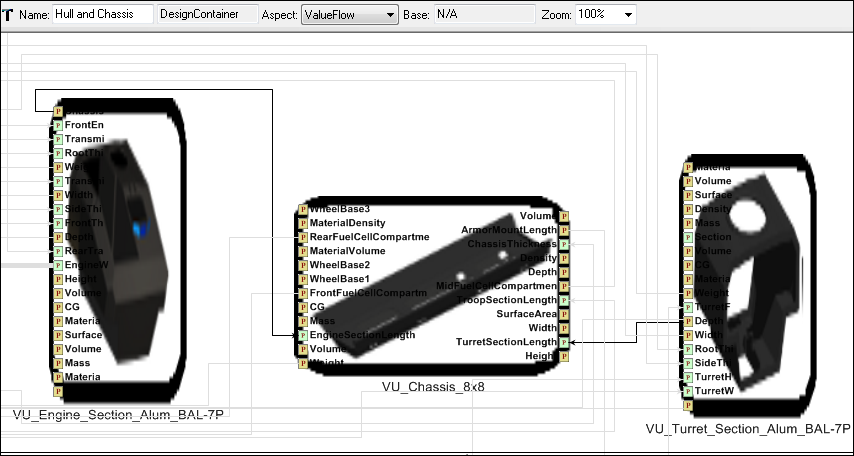
\includegraphics[scale=0.40]{Figures/cadParameter_VF.png}
\caption{Hull and Chassis Model.}
\label{fig:cadParameterVF}
\end{figure}
A Parameter object represents a static property of an object that can be tuned by a system designer at design-time. CADParameter is a specialization of Parameter. When a CAD model is built, the value of this object is used to set a specific parameter in the component's CAD representation. This is useful with parametrically-sizeable components, where the size of a component (or a feature of a component) depends on the size of another component that it is composed with. Figure \ref{fig:cadParameterVF} shows the Hull and Chassis portion of the IFV design space model. The VU\_Chassis\_8x8 component's TurretSectionLength and EngineSectionLength CADParameter objects get their Value attribute populated by VU\_Turret\_Section\_Alum\_BAL-7P's Depth Property object and VU\_Engine\_Section\_Alum\_BAL-7P's ChassisDepthMount Property object respectively.

\begin{figure}
\centering
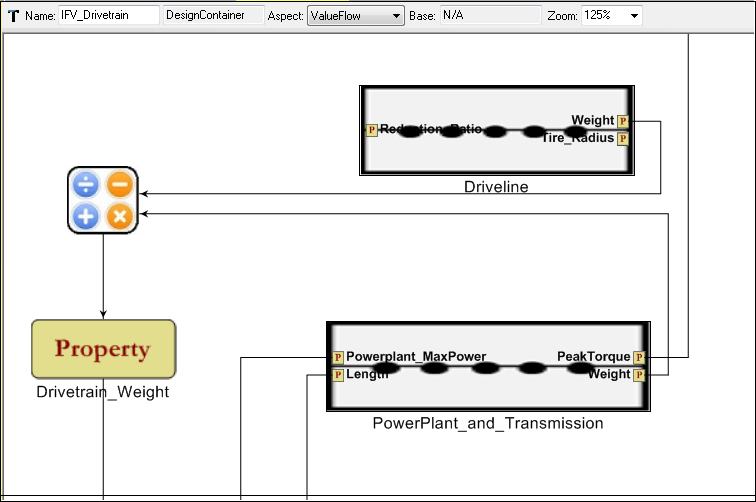
\includegraphics[scale=0.40]{Figures/Property_VF.png}
\caption{Drivetrain Design Space Model.}
\label{fig:propertyVF}
\end{figure}
A Property object represents a static property of an object or assembly. Properties of components cannot directly be changed at design time during design space model construction. Examples of Property are the weight of a damper and max power of a transfer case. Properties can be calculated from Parameters and other Properties using formula objects. Figure \ref{fig:propertyVF} shows the IFV\_Drivetrain design space model. In the figure, the Drivetrain\_Weight Property object is the sum of the Weight Property objects of Driveline and PowerPlant\_and\_Transmission. CADProperty is a specialization of Property. In practice, the value of a CADProperty must be calculated within a CAD tool, after which the result can be written back to the model. Examples of CADProperty in the current IFV model is the center of gravity and density of a Driver Hatch.

\begin{figure}[t]
\centering
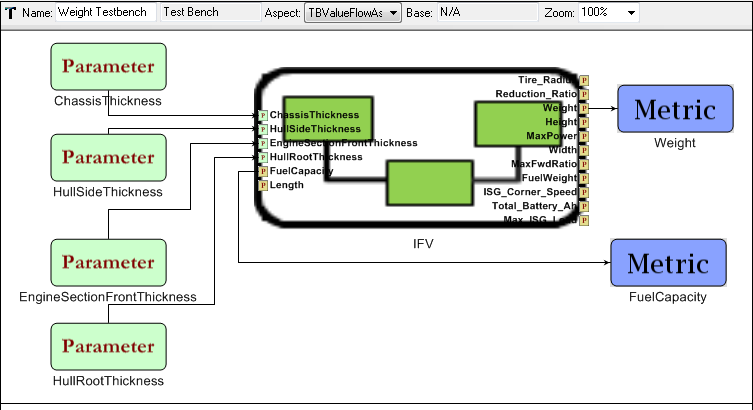
\includegraphics[scale=0.40]{Figures/Metric_VF.png}
\caption{Weight TestBench Model.}
\label{fig:metricVF}
\end{figure}
A Metric object is only used in test benches, test environments for testing composed systems, to capture outputs of running a test. A test bench is typically run on multiple designs of a system with the resulting metrics sometimes visualized in a GUI tool called Dashboard and compared across the designs. Figure \ref{fig:metricVF} shows the Weight TestBench model whose sole purpose is used for calculating the metric Weight and FuelCapacity of different IFV designs given an initial set of tunable input Parameter objects like HullSideThickness, ChassisThickness, etc.

\subsubsection{Using Formulas}
Formulas define relationship of connected value flow objects. There are two types of formulas in the CyPhy model used for describing calculation of property, parameter and metric quantities in the model. SimpleFormula are used for addition, multiplication, minimum, maximum, and geometric and arithmetic means. CustomFormula is a user defined algebraic expression using names of value flow objects or user define variable names. Incoming connections to a formula connects value flow objects  to the formula represents inputs used in the formula calculation. Outgoing connections represent output destinations to assign the calculated value to. A formula needs at least one input (incoming connection) and can be assigned to multiple value flow objects as well as other formulas.

A SimpleFormula has an attribute called Method which lets the user pick from the set of predefined mathematical functions to use on the input value flow objects. Addition, minmum, maximum, and average operations require that the units of input and output value flow objects be of the same dimension. If an input object doesn't not have an assigned unit, an attempt is made during evaluation process to automatically assign a compatible unit. For multiplication operations, the unit of inputs do not need to have the same dimesions. During evaluation process, the output's expected dimension is calculated based on the inputs' dimensions and checked against the actual dimension of the output's assigned unit. Figure \ref{fig:simpleformula} shows a SimpleFormula with inputs from Drivetrain, Hull and Chassis, and Turret assemblies and feeding the resulting sum to a Property object called Weight.
\begin{figure}[t]
\centering
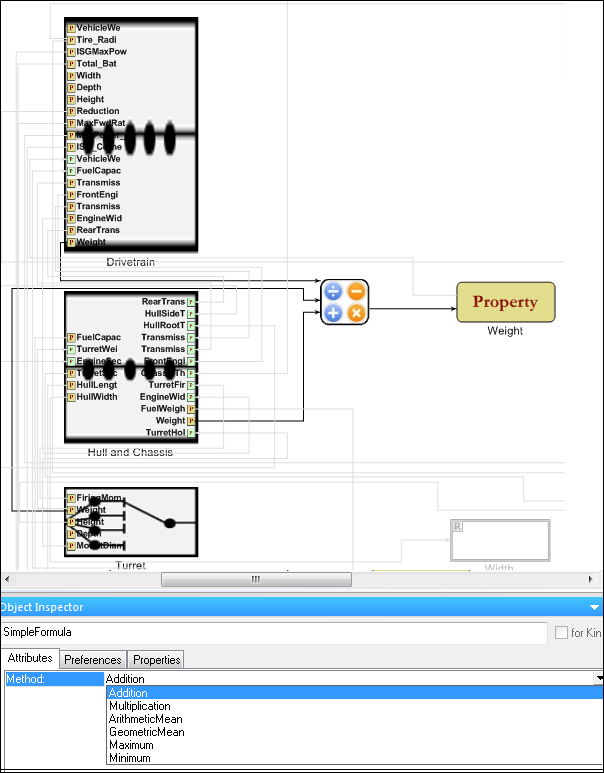
\includegraphics[scale=0.40]{Figures/simpleFormula_VF.png}
\caption{Simple Formula.}
\label{fig:simpleformula}
\end{figure}

A CustomFormula does not have any predefined operations. The user needs to type in a mathematical expression in the Expression attribute. During the evaluation process, third-party tool APIs (muParser) are called to parse and evaluate the expression. CustomFormulas are used primarily for surrogate equations in the IFV model. Units are not checked on CustomFormula intputs and outputs. The next subsection gives more detail on the syntax of CustomFormulas.

\paragraph{Formula Syntax}
CustomFormula supports algebraic expressions formed by combining constants, variables, mathematical operators and predefined functions. Variables can be the name of the input value flow object or the Variable Name attribute on the incoming value connection of a CustomFormula object. The supported operators and functions are listed in Tables \ref{tab:builtinfcntable} and \ref{tab:optable}. Built-in functions can support one more arguments, multiple arguments need to be seperated by commas and enclosed within a parenthesis. The arguments can be either constants or variables. The syntax for using an operator is (x operator y) where x and y are constants or variables.

\begin{table}
\parbox{.45\linewidth}
{
	\centering
	\begin{tabular}{ | l | l |}
	\hline
   Name & Num Argc \\ \hline    
    sin&1 \\ \hline
    cos&1 \\ \hline
    tan&1 \\ \hline
    asin&1 \\ \hline
    acos&1 \\ \hline
    atan&1 \\ \hline
    sinh&1 \\ \hline
    cosh&1 \\ \hline
    tanh&1 \\ \hline
    asinh&1 \\ \hline
    acosh&1 \\ \hline
    atanh&1 \\ \hline
    log2&1 \\ \hline
    log10&1 \\ \hline
    ln&1 \\ \hline
    exp&1 \\ \hline
    sqrt&1 \\ \hline
    sign&1 \\ \hline
    rint&1 \\ \hline
    abs&1 \\ \hline
    min&$>$1 \\ \hline
    max&$>$1 \\ \hline
    sum&$>$1 \\ \hline
    avg&$>$1 \\ \hline
   \end{tabular}
   \caption{Supported Functions}
   \label{tab:builtinfcntable}
   }
\hfill
\parbox{.45\linewidth}
{
	\centering
	\begin{tabular}{ | l | l |}
	\hline
    Name & Meaning \\ \hline    
    =&assignment \\ \hline
    \&\&&logical and \\ \hline
    ||&logical or \\ \hline
    <=&less or equal \\ \hline
    >=&greater or equal \\ \hline
    !=&not equal \\ \hline
    ==&equal \\ \hline
    >&greater than \\ \hline
    <&less than \\ \hline
    +&addition \\ \hline
    -&subtraction \\ \hline
    *&multiplication \\ \hline
    /&division \\ \hline
    $\wedge$&raise x to the power of y \\ \hline
  \end{tabular}
  \caption{Supported Operators}
  \label{tab:optable}
  }
\end{table}

Figure \ref{fig:customformula} shows two ways of writing a CustomFormula in the IFV\_DriveTrain design space model. The CustomFormula expression on the left used the name of input Property objects, Drivetrain\_Weight and PowerPlant\_MaxPower, along with constants. The example on the right used the VariableName attribute of the connections between CustomFormula and Drivetrain\_Weight and PowerPlant\_MaxPower Property objects. Notice that the attribute is displayed on both of the connections themselves. Both ways of writing the expression is valid and VariableName attribute should be used when there are multiple input value flow objects with the same name for a CustomFormula. 
\begin{figure}
\centering
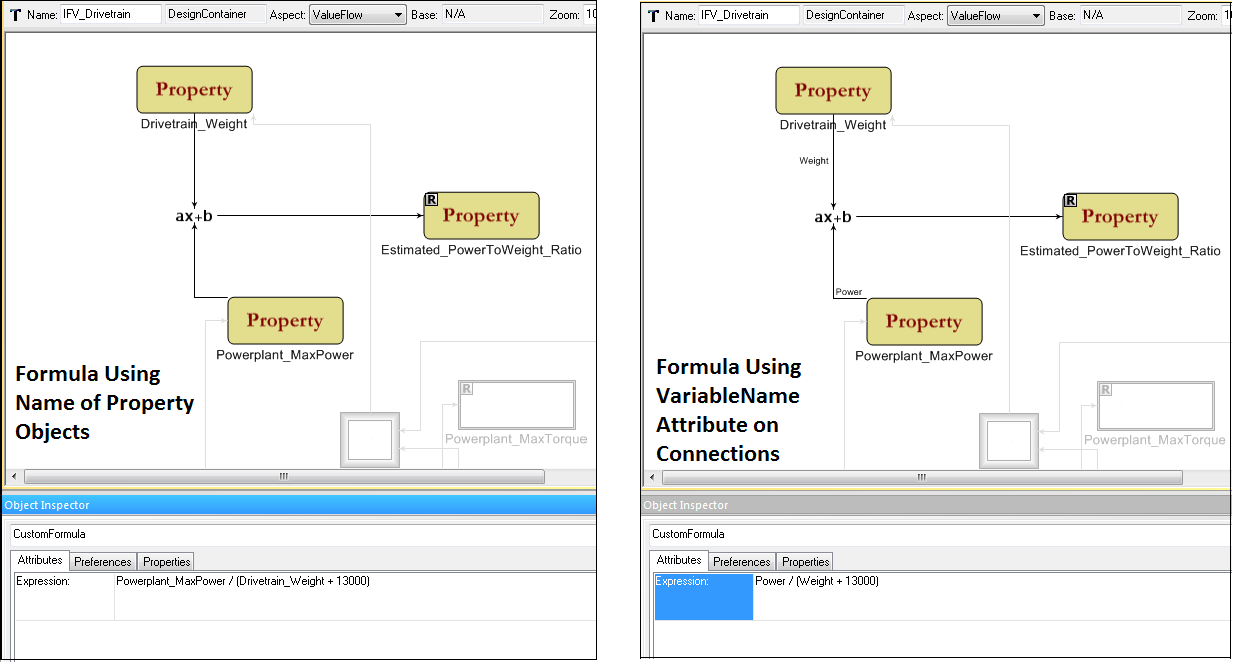
\includegraphics[scale=0.40]{Figures/customFormula_VF.png}
\caption{Custom Formula Using Name of Property Objects and VariableName Attribute on Connections.}
\label{fig:customformula}
\end{figure}


